\chapter{Raman amplification at 800 nm}
\label{chp:CLEO2010_Chapter}

We report the first experimental demonstration of Raman amplification in a fiber at wavelengths near 800 nm and propose its application to fast real-time optical sensing and imaging in this technologically important band. 

\section{Introduction}

Fast real-time optical sensors have numerous applications such as pattern-recognition, barcode reading, fingerprint matching, and face recognition, light detection and ranging (LIDAR), and industrial inspection and monitoring. They are equally important for studying dynamic phenomena in biological and biochemical processes. The central requirement for fast real-time operation is a signal integration time that is much shorter than the time scale of changes in the dynamic process. In practice, this requirement is very difficult to achieve because of the fundamental trade-off between sensitivity and speed; at high scan rates, fewer photons are collected during each integration time, leading to the loss of sensitivity \cite{goda2009serial,goda2008amplified,goda2009theory}. One prominent example of applications that require high scan rates and high detection sensitivity is in laser scanning fluorescence microscopy and two-photon microscopy used in applications such as mapping of neural activity in real time.

In conventional high-speed detection, photodetectors [e.g., photodiodes and photo-multiplier tubes (PMTs)] have to be cooled to reduce the thermal (electronic) noise level. However, cooling is undesirable as it requires a refrigeration unit to accompany the detector. Another technique used to increase the sensitivity is the use of a high-intensity illuminator. This approach is not suited for biological sensing as it can damage the sample especially in microscopy in which the light needs to be focused onto a very small field-of-view, resulting in extremely high optical power density (intensity). Optical amplification before the photon-to-electron conversion can overcome this fundamental challenge when the detection sensitivity is thermal noise limited. It eliminates the need for cooling and high-intensity illumination and therefore represents a powerful technique for detection of weak signals in spectroscopic and imaging applications. 

This so-called optical preamplification is exploited heavily in long-haul fiber-optic communications \cite{islam2002raman} where the severely attenuated optical signal would otherwise be drowned in the thermal noise of the optoelectronic converter (i.e., the photodiode and subsequent electronic amplifier). Optical preamplification then improves the sensitivity of the receiver by raising the weak signal above the thermal noise floor. Unfortunately, rare-earth (e.g., erbium) doped fiber amplifiers, the workhorse of fiber-optic communications, are limited to operation in the 1550 nm wavelength range -- a spectral region that is not suited for biological sensing because of the strong water absorption. Semiconductor optical amplifiers (SOAs) can operate at other wavelengths; however, they suffer from high noise figures and hence are not well suited as preamplifiers. 

The 800 nm band (700 -- 900 nm) is important for biomedical applications because of the availability of the popular Ti:Sapphire lasers and also because it permits much larger penetration depths in tissue. The latter is due to a compromise between Rayleigh scattering (that increases at shorter wavelengths) and water absorption (that increases at longer wavelengths) in this wavelength band. Compared to shorter wavelengths, the 800 nm band is also important for fluorescence microscopy with fluorescent dyes or quantum dots as background noise due to auto-fluorescence is greatly reduced. The low absorptivity and scattering of light in tissue in this band enable in vivo imaging and subcellular sensing applications.

\section{Advantages of Raman amplification}

Compared to different approaches to optical amplification, stimulated Raman scattering (SRS) \cite{islam2002raman} provides several advantageous over other methods such as rare-earth doped fiber amplifiers and SOAs. First, gain is possible at any wavelength as long as a pump is available at a frequency blue-shifted from the signal by the optical-phonon vibrational frequency. Second, a broad and flexible gain spectrum can be obtained by using multiple pumps. Finally, Raman amplifiers have a lower noise figure than rare-earth doped fiber amplifiers and SOAs \cite{islam2002raman}. It is also ideal for amplified dispersive Fourier transformation \cite{goda2009serial,goda2008amplified,goda2009theory}, a technique for fast real-time spectroscopy and imaging. 

In this chapter, we report, to the best of our knowledge, the first experimental demonstration of Raman amplification in an optical fiber in the 800 nm band. Furthermore, we show the first measurement of the Raman gain coefficient near 800 nm. Because of limited pump power available and the large losses in the fiber used in these experiments, net amplification could not be achieved. However, we show that with higher pump powers than what was available in our experiment and which are within the range of commercial amplified Ti:Sapphire lasers, significant net gain can be achieved. 

\section{Experimental demonstration}

To demonstrate Raman amplification, we constructed the experiment (for forward pumping) shown in Figure \ref{fig:CLEO2010_Figure1}. A weak continuous-wave solid-state laser at 808 nm (CrystaLaser) is the amplifier input (Stokes field) that enters a 5 km long Ge-doped silica-core single-mode fiber with a mode-field diameter of 4 $\mathrm{\mu}$m (Nufern) via a fiber coupler. The small mode-field area increases the nonlinear interaction in the fiber. The fiber is forward-pumped by a continuous-wave frequency-tunable Ti:Sapphire laser at around 788 nm (KM Labs). The pump power coupled into the fiber is about 200 mW. The spectrum of the output Stokes field is measured with an optical spectrum analyzer. 

\begin{figure}[htb!]
\centering
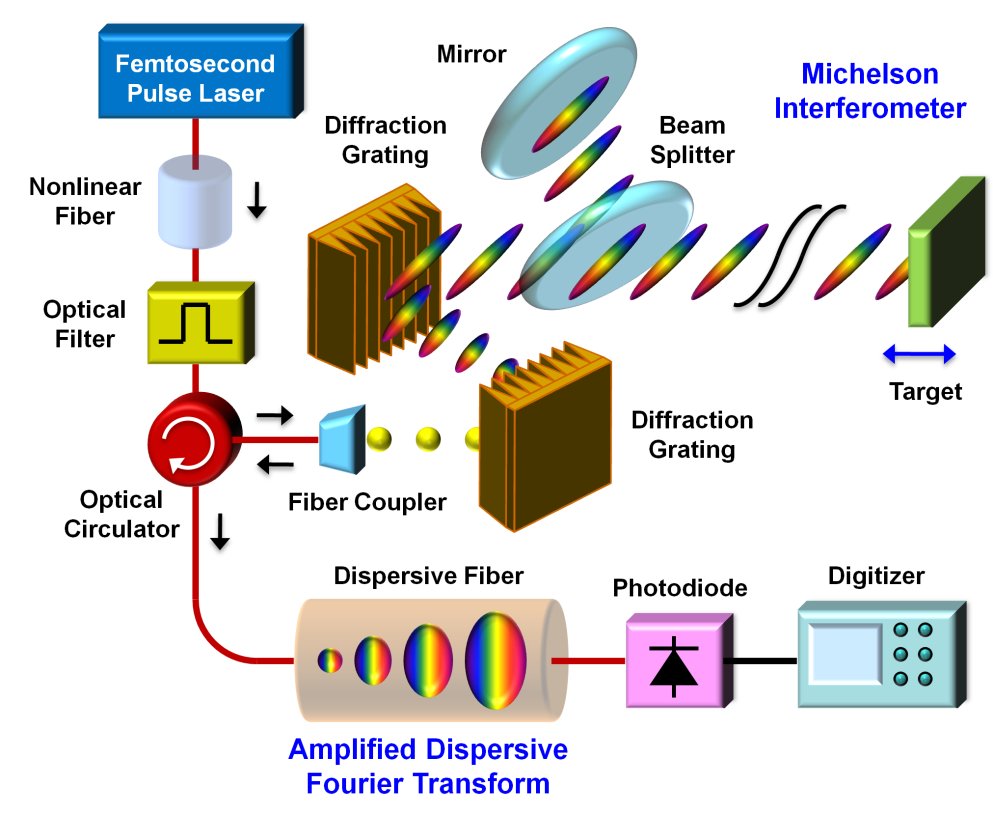
\includegraphics[scale=1]{CLEO2010/Figure1.png}
\caption{Distributed Raman amplification in a Ge-doped silica-core single-mode fiber. The input Stokes field is amplified by stimulated Raman scattering (SRS) in the fiber. The amplified Stokes field is detected by the optical spectrum analyzer.}
\label{fig:CLEO2010_Figure1}
\end{figure}

Experimental results are shown in Figure \ref{fig:CLEO2010_Figure2}. First, the pump field was turned on and off to isolate the effect of Raman amplification. Then, with the pump on, the Stokes field was turned on and off to observe the noise level of the pump field. Finally, with the Stokes field off, we varied the pump power and observed the signal at the Stokes wavelength to observe any amplified spontaneous emission (ASE) arising from the SRS process. As shown in Figure \ref{fig:CLEO2010_Figure2}, any ASE was masked by the broadband fluorescence from the Ti:Sapphire crystal. The presence of the pump field in the fiber increased the Stokes power by 4.7 dB, indicating Raman amplification in the fiber. The contribution of the fluorescence from the Ti:Sapphire crystal to the amplified Stokes field is negligible as the difference in power between them is more than 10 dB. To validate Raman amplification in the fiber and exclude other possibilities, we measured the Stokes field before the fiber with and without the pump field and confirmed no difference in the Stokes field intensity between the two cases. 

\begin{figure}[htb!]
\centering
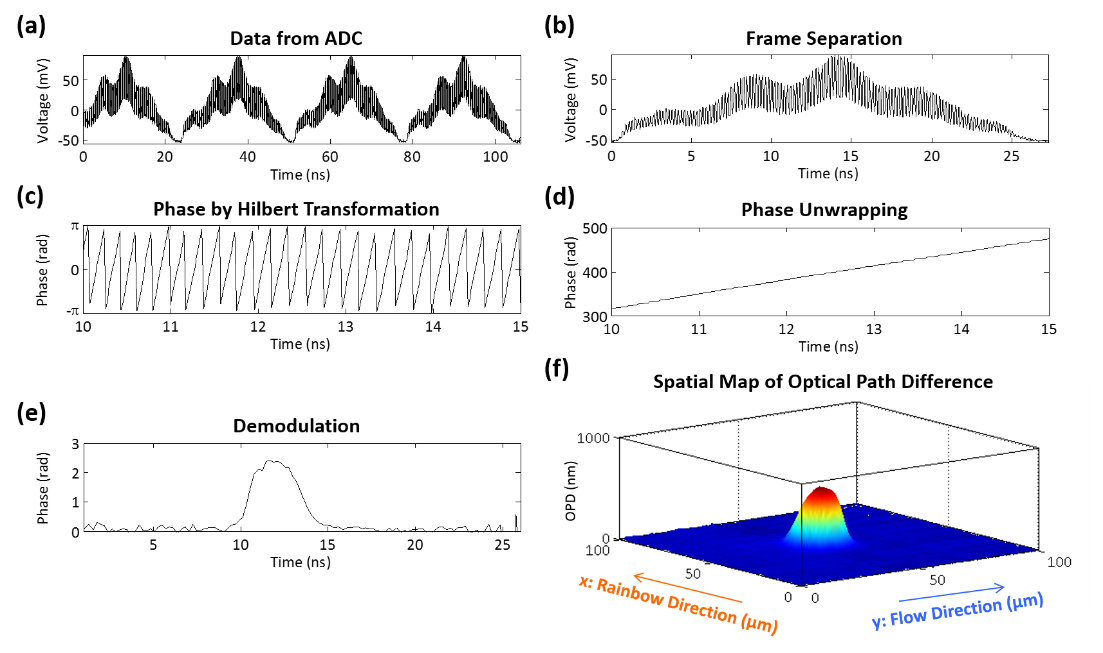
\includegraphics[scale=1]{CLEO2010/Figure2.png}
\caption{Experimental demonstration of Raman amplification at 808 nm in a single-mode fiber. The presence of the pump field amplified the Stokes field by 4.7 dB.}
\label{fig:CLEO2010_Figure2}
\end{figure}

We also measured the Raman gain spectrum by tuning the pump while keeping the Stokes wavelength fixed (Figure \ref{fig:CLEO2010_Figure3}). The obtained gain was found to reach a value of $5.4 \times 10^{-14}$ m/W at about 30 nm or 14 THz off-set from the pump (the spectral range in our measurements was limited by the tunability range of the Ti:Sapphire laser). From independent measurements, the loss coefficient of the fiber is found to be $7.8 \times 10^{-4}$ m$^{-1}$ or -3.4 dB/km (approximately equal for both the Stokes and pump wavelengths). Simulation results indicate that if pump powers higher than 0.2 W achievable in our experiment are available, then net gain as high as 30 dB can be achieved. The 1 W pump level required for this is achievable with a commercially available amplified Ti:Sapphire laser. 

\begin{figure}[htb!]
\centering
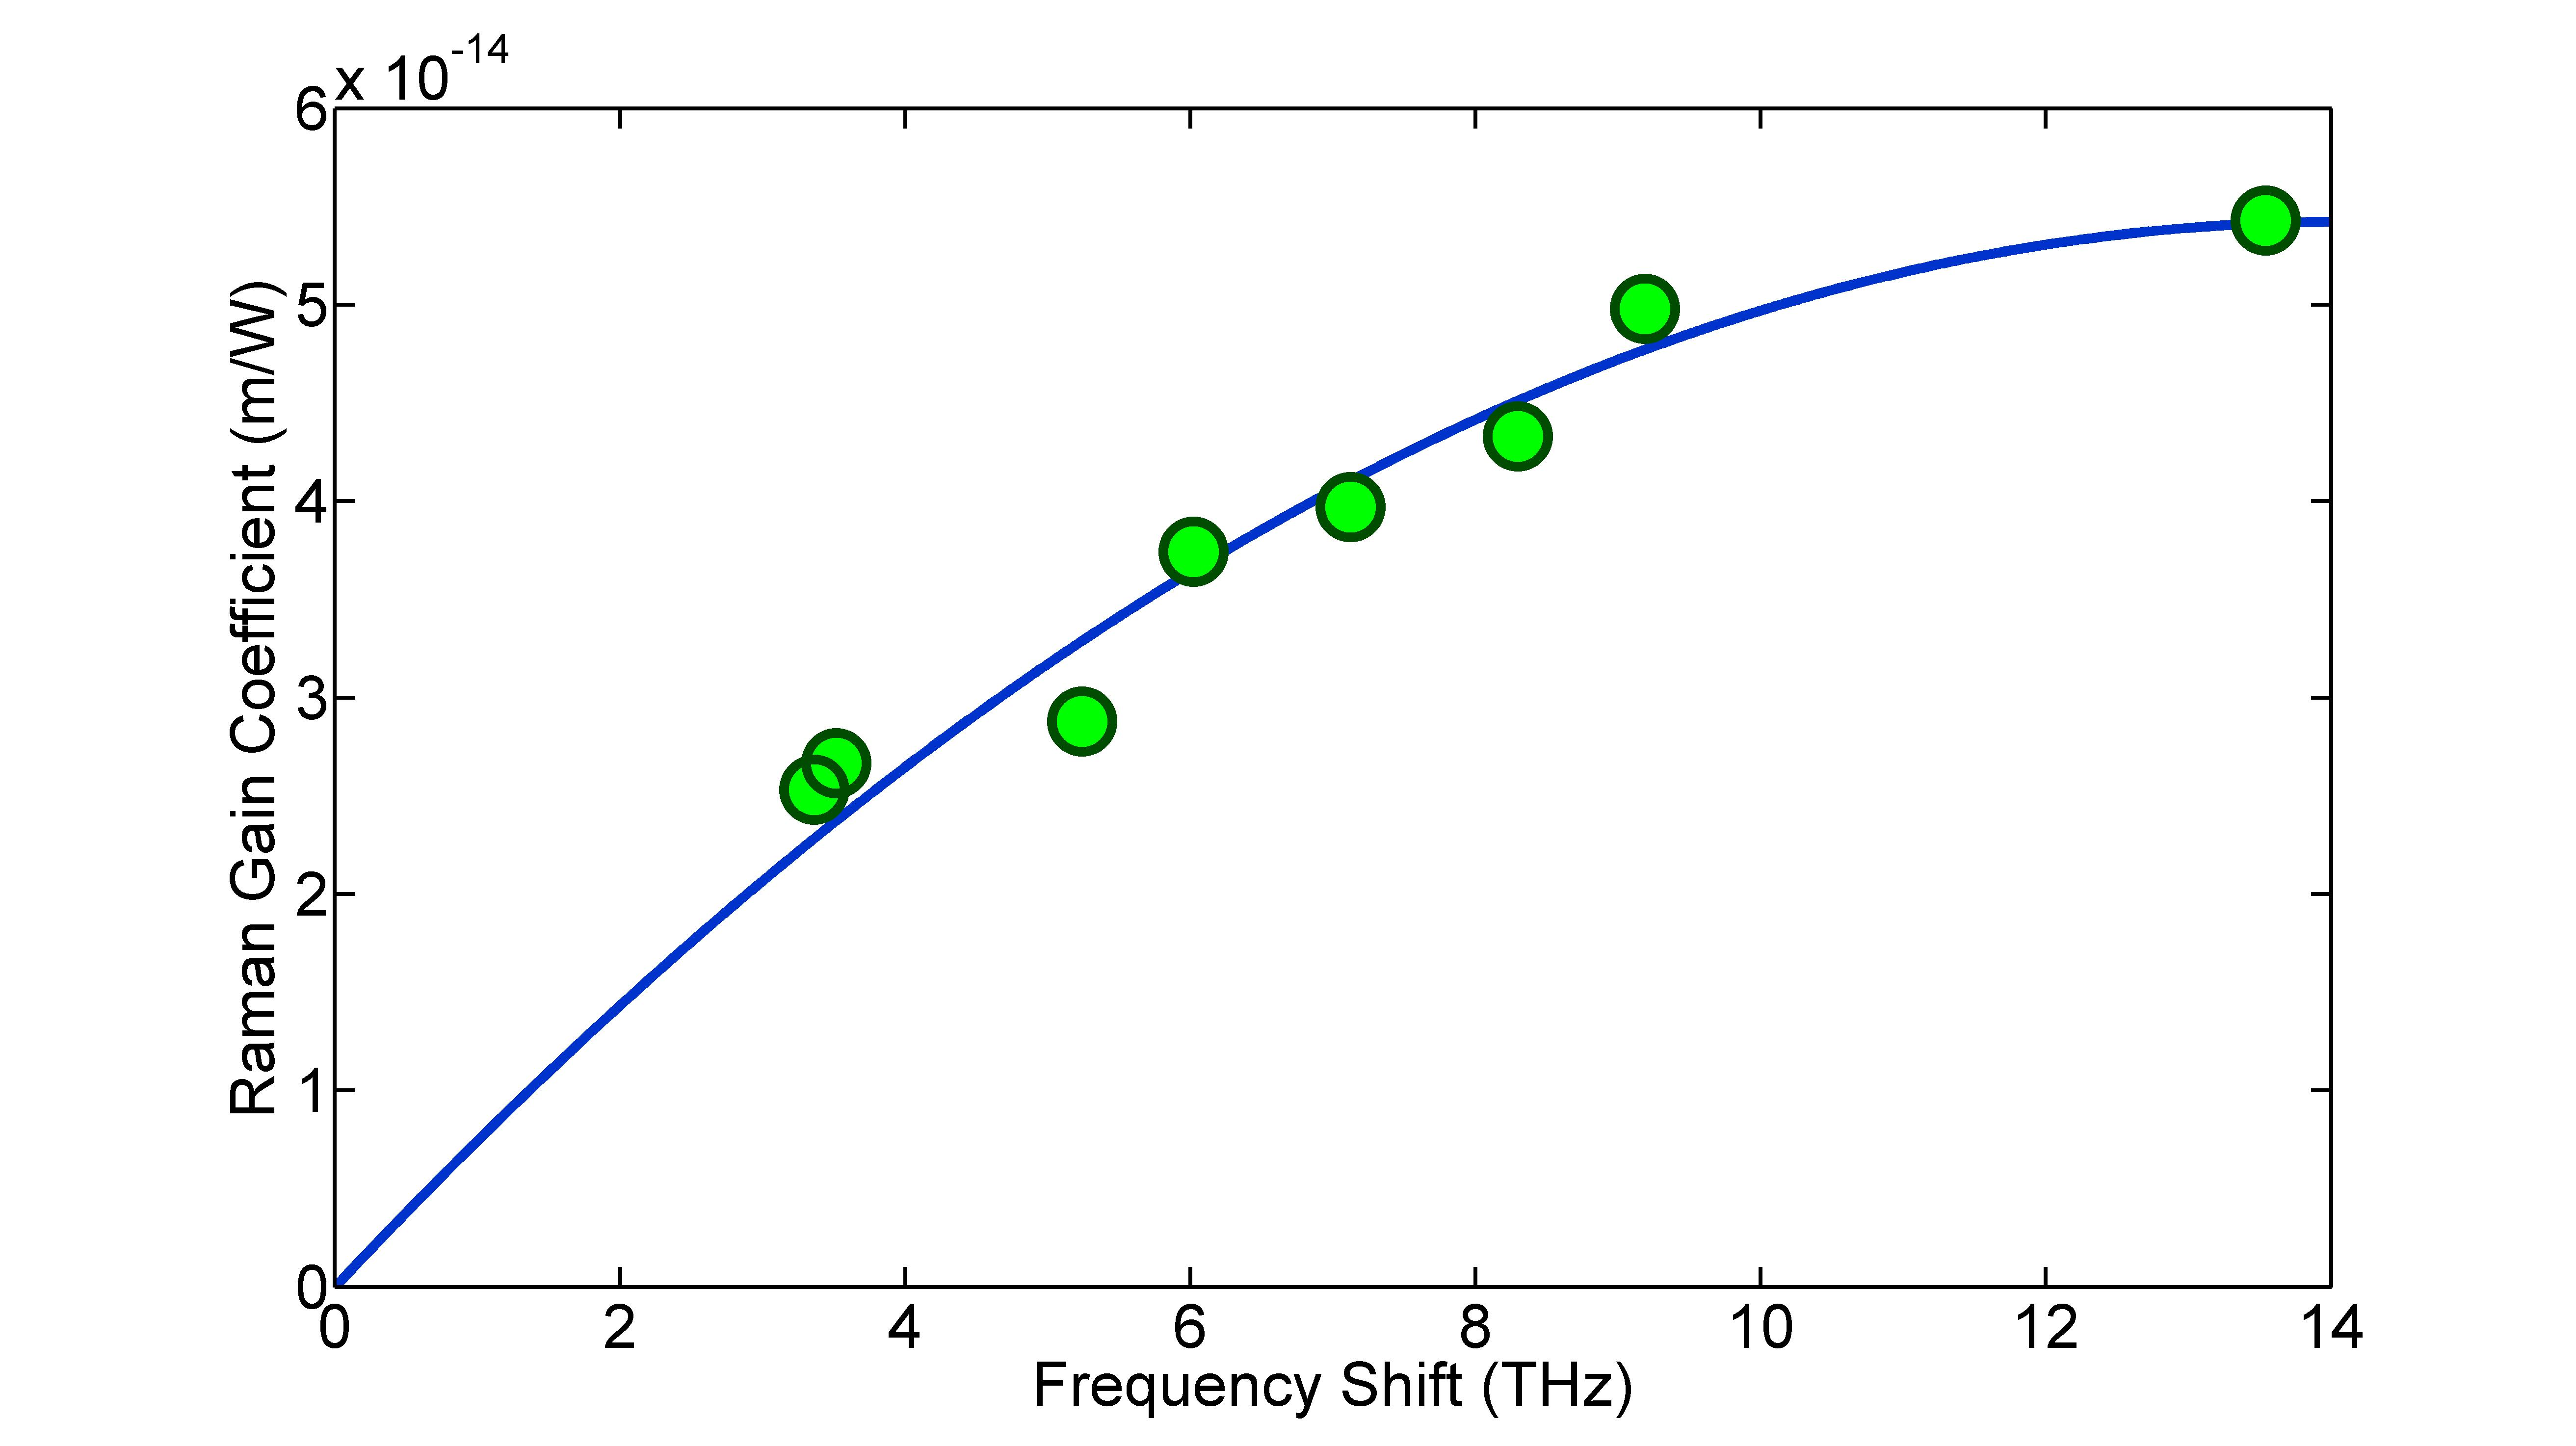
\includegraphics[scale=0.11]{CLEO2010/Figure3.png}
\caption{Raman gain spectrum at 808 nm Stokes wavelength. At a pump wavelength about 30 nm from the Stokes wavelength (or a frequency shift of 14 THz), the Raman gain reaches a maximum of $5.4 \times 10^{-14}$ m/W.}
\label{fig:CLEO2010_Figure3}
\end{figure}
